\chapter{Supervised learning approach}
\label{mrcnn_chapter}
In this section we introduce Mask {R-CNN} \cite{DBLP:journals/corr/HeGDG17} as our primary supervised model for solving Euclidean construction problems, describe how to train it and how to obtain Euclidea actions from Mask {R-CNN} model predictions.

\begin{figure}[h]
\centering
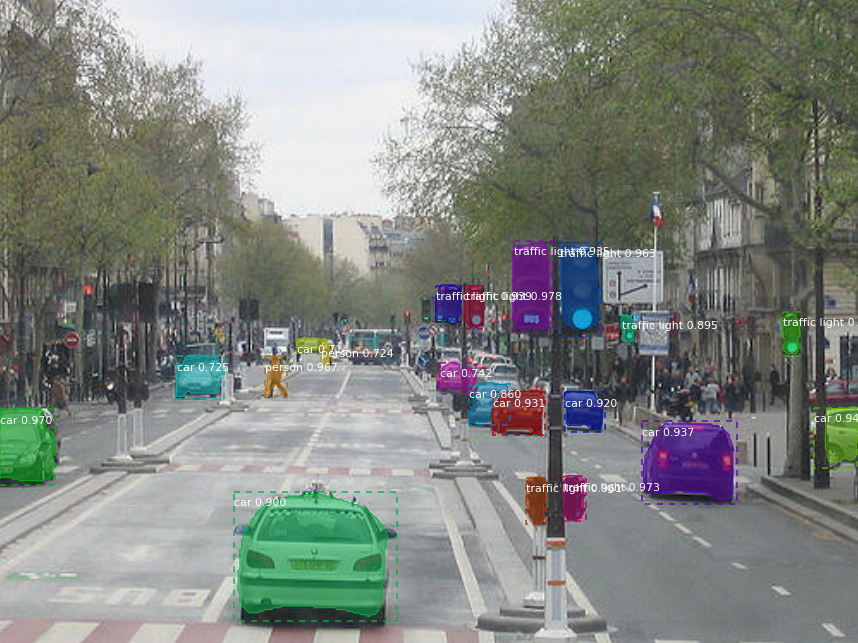
\includegraphics[width=140mm]{img/mask_rcnn_example.png}
% Rozměry také není nutné uvádět.
\caption{Example of a detection with the Mask {R-CNN} model. Source: \cite{matterport_maskrcnn_2017}}
\label{mrcnn_example}

\end{figure}


\section{Mask {R-CNN}, review}
Mask R-CNN is a deep neural network used for, detection, classification and segmentation of objects in images and videos. The input is an image and the output is a set of bounding boxes, segmentation masks and class labels for each detected object instance in the image. Example output is shown in Figure \ref{mrcnn_example}
\newline \newline
Mask {R-CNN} first computes image features with a convolutional backbone, usually the ResNet backbone. Followed by two stages of Mask {R-CNN}. The first stage is a deep convolutional network with Region Proposal Network, which proposes regions of interest from the features computed by the backbone. The second stage uses the ROI pooling layer and predicts class, bounding box and mask for each ROI.

\begin{figure}[h]
\centering
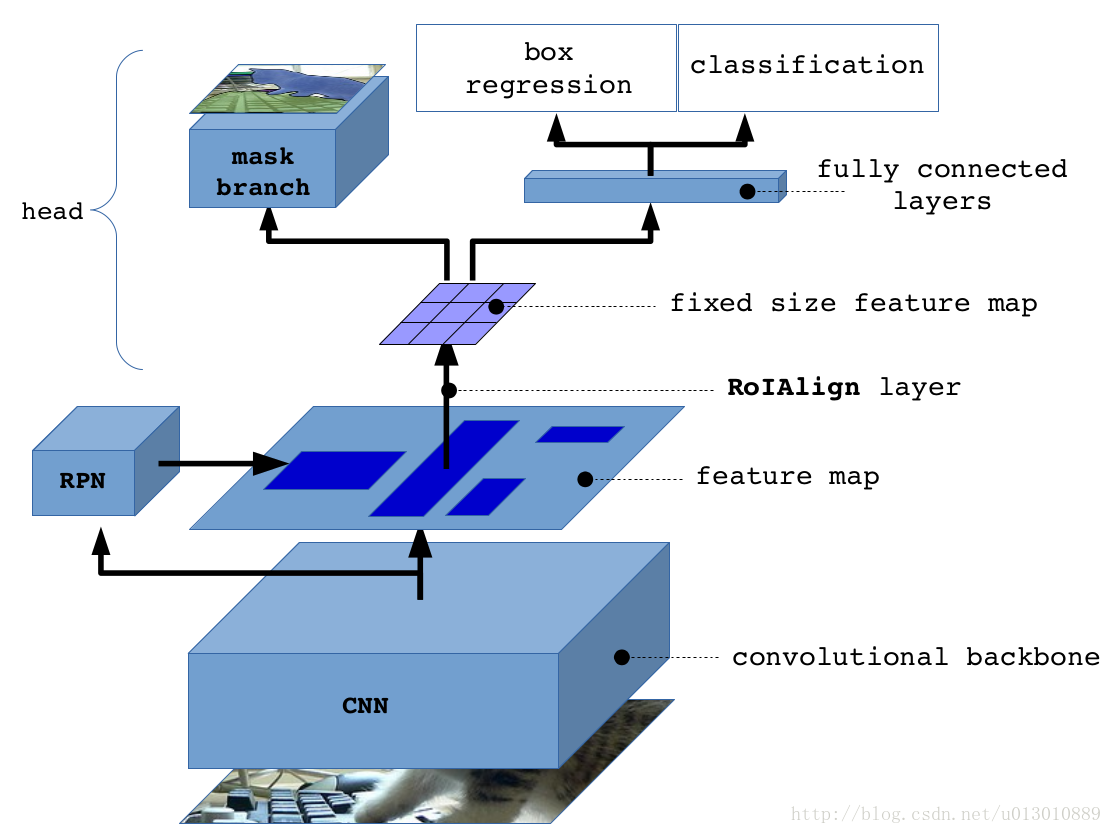
\includegraphics[width=140mm]{img/mask-rcnn_schema.png}
\caption{Diagram of the Mask {R-CNN} model, the CNN backbone, the ROI proposal network and head mask layers. Source: \cite{mrcnn_schema}}
\label{mrcnn_example}

\end{figure}
\section{ Mask R-CNN for solving geometric constructions}
In Figure \ref{our_approach_schema} we can see the schema of our approach. We generate the training data as we go through Euclidea levels. We solve levels by following a predefined construction that is recomputed to a current instance in the generation process (see Section \ref{degen_criteria}). Each application of a Euclidea tool corresponds to one sample in the training data. To train Mask {R-CNN} to solve geometric constructions, we have to create training data that represent tool usage, and we have to adjust outputs of the network to work with the Euclidea-like environment. 
\newline \newline
We denote each application of a tool in our environment as an ``action''. For this purpose, we assign each tool an index, e.g.~ 1 for Line tool, 2 for Circle tool, etc. An action is then represented by the index of the tool and the corresponding number of click coordinates (see Section \ref{Euclidea_tools}). For example, the Line tool needs two action clicks, which represent two points on the line. Next, we will describe how to generate training data for Mask {R-CNN} and how to infer actions from those masks. 
\begin{figure}[h]
\centering
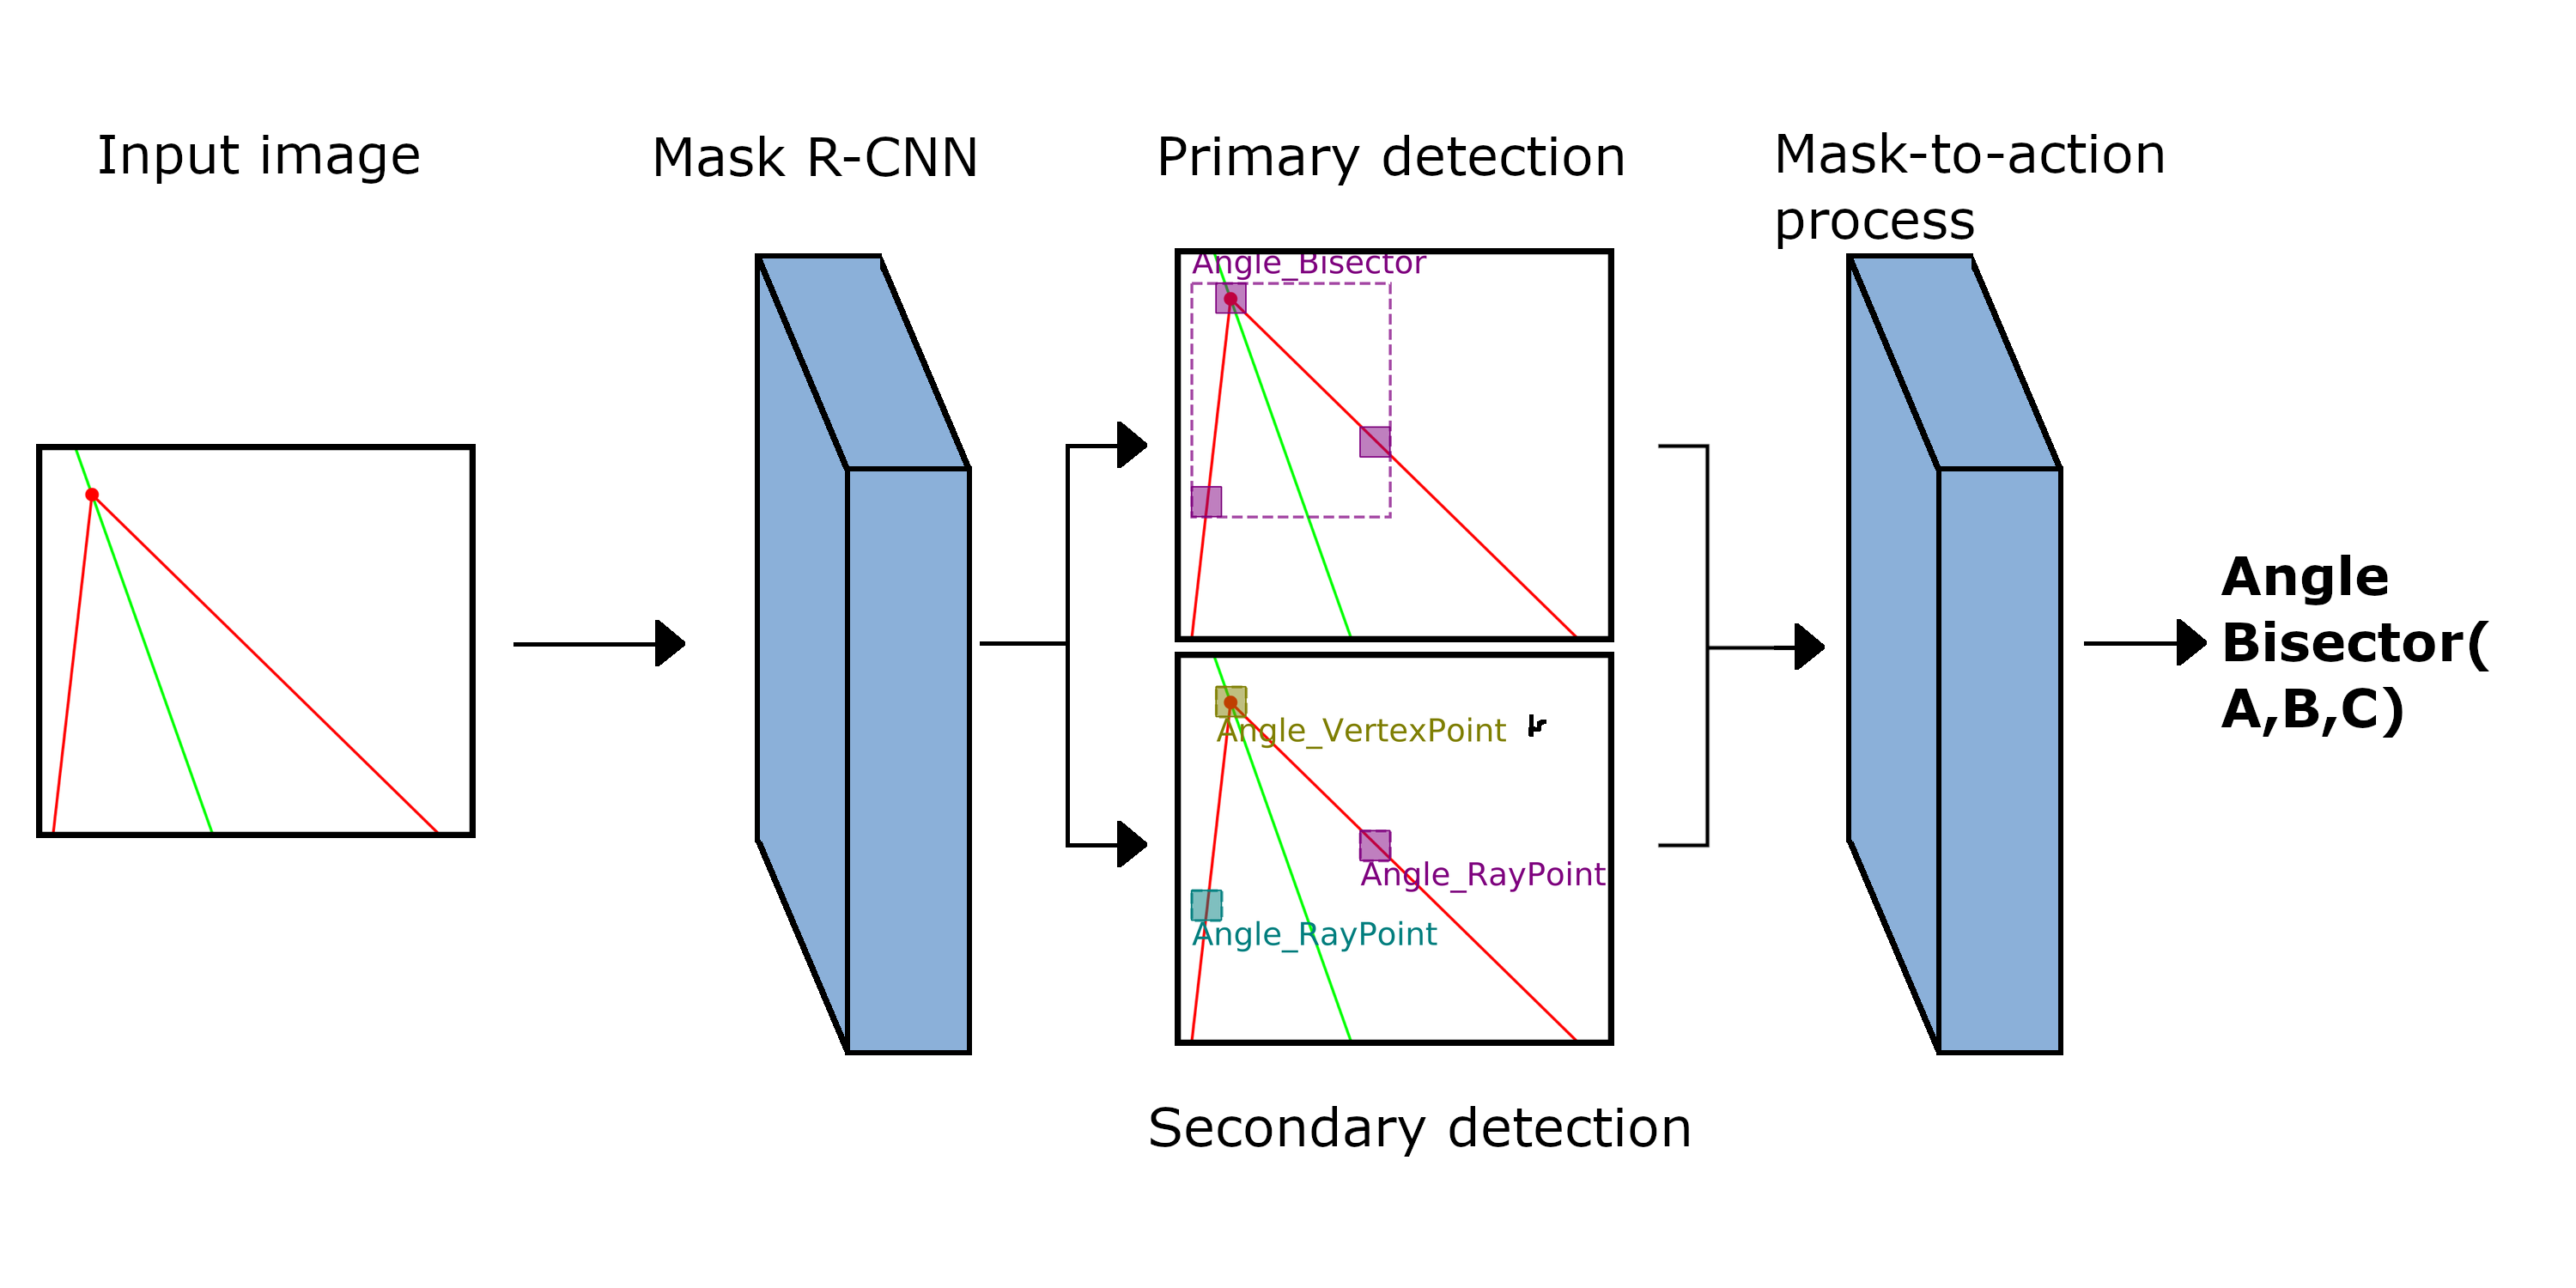
\includegraphics[width=140mm]{img/approach_schema.png}
\caption{Diagram of our approach. The input is an image of the scene, which is run through Mask {R-CNN}. The input image contains an RGB image with the current state of the construction in the red channel and the remaining goal in the green channel. The results are primary and secondary detections, which are then used to obtain an action tool for Euclidea. Note that there is no head for predicting primary and secondary detections. Instead, both are predicted with the same head and sorted to primary and secondary detections by the prediction id. How the Mask-to-action process works is described Sections \ref{action_to_mask} and \ref{position_dependent_pars}}
\label{our_approach_schema}

\end{figure}
\subsection{Action to mask}
\label{action_to_mask}
\begin{figure}[h]
\centering
\begin{tabular}{c c}
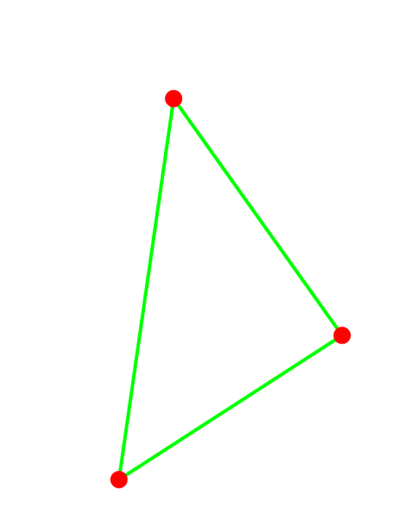
\includegraphics[width=0.45\textwidth]{img/ExampleTrainingData/01_01_input.png} &
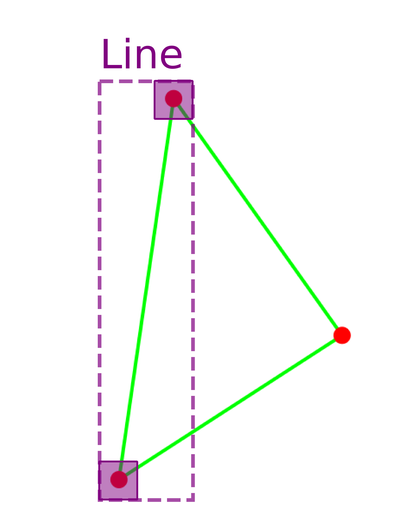
\includegraphics[width=0.45\textwidth]{img/ExampleTrainingData/01_01_primary.png} \\
a) Input & b) Primary detection
\end{tabular}
\caption{A sample from training data for level \textit{Alpha-01}: Tutorial for the Line tool, connects points. Both parts contain the current state (red), remaining goal (green).
Input for the model is on the left and target mask (purple in this case) for the Line tool with respective bounding box on the right. The mask contains two areas for each endpoint of the triangle side, representing click coordinates for the tool. The Line tool does not have position-dependent parameters. Hence the secondary detection is empty and not shown.}
\label{training_data_primary_01_01}
\end{figure}
We represent the input of the Mask {R-CNN} as an image of the scene with current state in the red channel and the remaining goal in the green channel. In our experiments, we also add extra channels representing history (see Section \ref{history_channel}). The $n$-th history channel represents the state of the scene $n$ steps before the current state.
\newline \newline
A target is a pair of an object type and its location, represented as a mask of the object. Object type corresponds to the tool that is used in the step. The target mask is the mask of each point click contained in the step.
These sub-masks are squares around the click location. Also, some tools have a line as its argument; passing a line argument can be a mask of a single click on the line or a mask of the whole line. Figure \ref{training_data_primary_01_01} shows an example of input and output.

\subsection{Tools with position-dependent parameters}
\label{position_dependent_pars}
\begin{figure}[h]
\centering
\begin{tabular}{c c c}

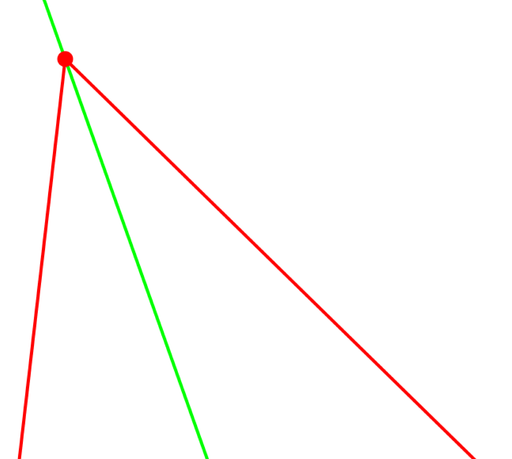
\includegraphics[width=0.3\textwidth]{img/ExampleTrainingData/02_02_input.png} &
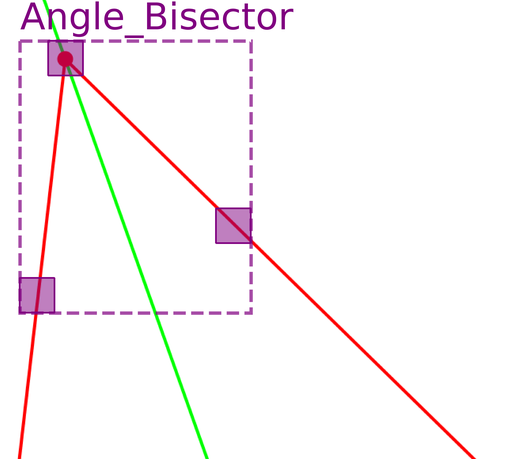
\includegraphics[width=0.3\textwidth]{img/ExampleTrainingData/02_02_primary.png} &
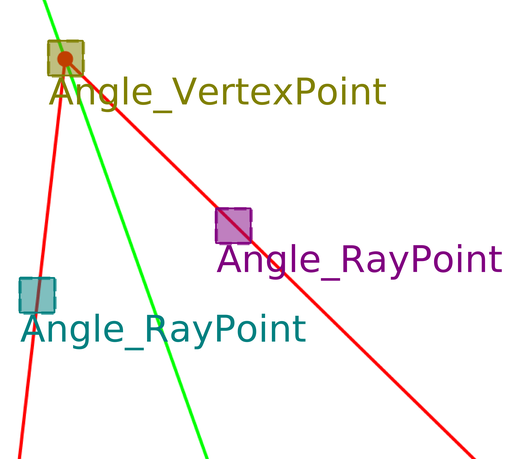
\includegraphics[width=0.3\textwidth]{img/ExampleTrainingData/02_02_secondary.png} \\
a) Input & b) Primary detection & c) Secondary detection
\end{tabular}
\caption{Sample from training data for level \textit{Beta-02}. All three parts contain the current state (red), the remaining goal (green).
Subfigure b) is a primary detection of Angle Bisector tool(purple) c) are three secondary detections: 2x angle ray point (purple, turquoise) and 1x angle vertex point(dark-yellow).}
\label{training_data_primary_02_02}
\end{figure}
Encoding clicks like in the previous subsection is not sufficient for most tools where tool parameters are position-dependent. For example, the Circle tool has two parameters: a circle center and a point on the circle. For such tools, we also have to distinguish these points. Therefore we have to add an additional target. For the Circle tool, for example, we also detect the circle center and the circle radius-point. In this thesis, we call the Circle tool detection the primary detection, and the detection intended for parameter order the secondary detection. We can see an example of primary and secondary detections in Figure \ref{training_data_primary_02_02}.
\newline \newline
Another special case is the Compass tool. We know that $\compass(A, B, C) = \compass(B, A, C)$ where $A$, $B$, and $C$ are any valid inputs from the definition of the Compass tool. This is related to the number of degrees of freedom for each tool discussed in Section \ref{degrees_of_freedom}. If a tool has this property, we can use the same object type for $A$ and $B$. This will reduce the number of object classes and also improve the problem trainability. The reason for it is that there can be multiple very similar scenes in training data that have different permutations of such points that can be switched. Then we could get to a situation where the points may be indistinguishable.


\subsection{Reducing ambiguity}
An ambiguity in a construction occurs when the next step is, for example, a random point on a given line. We would like to have every possible point on the line that does not lead to a degenerated construction in the training data. However, computing areas where points could be is extremely time-consuming. To check all degeneration criteria for a single example, we would have to check {$O(n^2)$} rules, where $n$ is the number of points in the scene. Furthermore, those areas where we cloud create a point are not even continuous, so we would have to test many points in space. On top of that, when adding multiple random points, we would have to solve whether a pair, triplet, or n-tuple of random points lead to valid construction, which would lead to exponential numbers of degeneration checks.
\newline \newline
Therefore, we reduce the ambiguity as much as we can. For example, in level \textit{Alpha-12} the goal is to find the center of a given circle. The order of the construction is:
\begin{enumerate}
  \item Angle bisector between 2 random points on the circle.
  \item Another angle bisector between 2 random points on the circle.
  \item Intersection of those angle bisectors is the circle center.
\end{enumerate}
When we want to minimize ambiguity, we need just 3 random points. It is also beneficial to fix the relative positions of these points.  We choose to fix those 3 random points to sections that correspond to points {$(1,0)$, $(-1,0)$, $(0,1)$} on the unit circle. If we do not address these ambiguities, predictions can look like in Figure \ref{mrcnn_example_01_12}, where we can see many point candidates. Having that many point candidates significantly lowers the inference accuracy.  
\newline \newline
\begin{figure}[h]
\centering
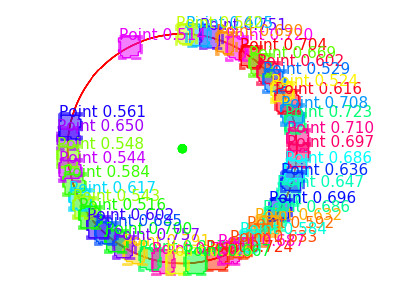
\includegraphics[width=120mm]{img/GenerationExamples/NotFixedAmbiguityCircleCenter.png}
\caption{level \texit{Alpha-12}: Find the center of a given circle. In the construction of this level, we have to create three random points on the circle, but the Mask R-CNN proposes many points due to ambiguity in training data used for training of the model. Due to the number of predicted points, we cannot use prediction like this in inference.}
\label{mrcnn_example_01_12}
\end{figure}
\section{Solving geometric constructions}
In this section we describe how we obtain actions for our Euclidea environment from the Mask {R-CNN} model.
\subsection{Mask to action}
We cannot measure the success of the model directly by its loss function. Instead, we have to measure the accuracy of level completion in the Euclidea environment. In the experiments section (see Section \ref{on_the_fly_section} and Figure \ref{on_the_fly_gen_loss}), we will see that a higher loss model can have better completion accuracy. However, we still have to monitor the loss since it should decrease during training regardless of its value.
\newline \newline
To solve Euclidea levels, we have to transform Mask {R-CNN} output to suit our environment input. The output of the model is a mask and the object type. The final layer of the Mask {R-CNN} produces a heat map, which is a probability map that gives each pixel a probability whether it is part of the mask or not. The heat map is then transformed into a mask by applying a $>0.5$ threshold to each element of the heat map. The heat map is used to create actions suitable for the environment.
\newline \newline The most straightforward actions to create are actions that correspond to the Line tool and Perpendicular Bisector tool, because these tools have a single degree of freedom. Hence we do not have to deal with  the order of the arguments. Both tools take two arguments. We take the two most probable points from the heat map that are to too close to each other. We use the same minimal distance threshold as the minimal point distance in degeneration. To find these two points, we use our version of the RANSAC algorithm \cite{Fischler81}.
\newline \newline
Now, let us describe more complicated tools. As an example, let us consider the Angle Bisector tool, which has 3 input parameters. Detection of this tool should have 4 detection outputs from Mask {R-CNN}: 1 primary and 3 secondary detections.
The primary detection is the detection of the angle bisector. Secondary detections are detections for the individual points: 
one angle vertex point and two angle ray points (see Figure \ref{training_data_primary_02_02}).
\newline \newline
To execute the tool, we have to determine the correspondence between the primary and the secondary detection.
We can obtain 3 point coordinates from the primary detection in the same way as above with the Line tool. We can also get 3 points from 3 secondary detections, each giving us one point. Each point from the primary detection corresponds to some point in the secondary detection, but these points do not exactly align. The point correspondence is then determined by minimizing distances between the primary and the secondary points (each point has to be used exactly once).
\newline \newline
\label{inferene_highest_score}
Now we can create an agent that can solve Euclidea levels. In the previous paragraph, we have described how to get an action from a single prediction.  However, Mask {R-CNN} can predict multiple actions. Mask {R-CNN} also predicts a score for each object, representing the confidence of the prediction.  For now, we can use the prediction with the highest score.  Detections with lower confidence may also be useful, and we will return to them in the next chapter.  However, multiple detections complicate the assignment of the secondary predictions. Mask {R-CNN} does not connect different detections, so we can have more secondary detections than points in the primary detection. We can still use the approach we mentioned previously, just for the assignment we no longer use each point exactly once, instead once or not at all. 
Then the agent does the following:
\label{top_score_inference}
\begin{algorithm}[h!]
\SetAlgoLined
 %\KwData{this text}
 \KwResult{Test level inference: True if level completed, False otherwise.}
 Initialize a level\;
 \While{level not complete}{
  $s \gets$ current state of the level\;
  $p \gets model.predict(s)$\;
  \If{predictions $p$ are empty}{
   \Return False\;
   }
  $a \gets$ action from $p$ with highest score\;
  execute $a$
 }
 \Return True\;
 
\caption{Inference: Top score prediction}
\end{algorithm}

In Table \ref{EuclideaExample-Network}, we can see an example solution of the geometric problem solved using top score predictions.

\subsection{Incomplete detections}
There are instances of levels with incomplete detections. A detection is incomplete if there are not enough points in the primary or the secondary detection. If there are not enough primary points, we cannot determine any action. For secondary points, we can determine as many points as possible, and then the rest of the points can be randomly assigned. Applying a random assignment is frequently used in inference, mostly for the Circle tool. Many constructions use a sequence of $\circletool(A, B)$ followed by $\circletool(B, A)$ to obtain equilateral triangle, perpendicular bisector, midpoint of a segment, 60$^{\circ}$ degree angle, etc. During inference of this situation based on data from the first detection, we have to construct either $\circletool(A, B)$ or $\circletool(B, A)$ and the second detection has to construct the other circle. When we go through Euclidea levels while creating the training data, we have to choose which step we do first.
Furthermore, because we generate level instances randomly, there can be multiple similar level instances during training that choose different moves, i.e.~there are two samples in training data that have the same primary detections but different secondary detections. During training, those secondary detections may cancel each other out resulting in the primary detection without the secondary one. However, as mentioned above, we can use any action defined by the detected primary actions. This effect occurs mostly for the Circle tool, but it can occur for other tools as well.
\subsection{Opposite corner detection}
Some detections may miss click coordinates even in the primary detections. However, the prediction of a bounding box can still be predicted correctly. If a tool has 2 arguments, we can find another point in this situation with point reflection. We reflect the detected point with the center of symmetry in the center of the bounding box. The bounding box for the training data is a minimal bounding box containing the mask in the training data. Hence when we expect the output to have 2 click coordinates, one point is in a corner, and the other is in the opposite corner of the bounding box.

\section{Other models}
Before we experimented with Mask {R-CNN}, we tried models that predict action click coordinates straight from images. The output of the model were coordinates, not a mask. We used a convolutional network with few densely connected layers and two output layers: a softmax layer that predicted the tool index and a layer with 6 outputs representing x and y coordinates of 3 points. The activation function for the layer predicting coordinates was the sigmoid activation multiplied by the window size (size of the input image). Hence all predictions were valid coordinates within the image. However, this model had problems even on simple levels like \textit{Alpha-01}. It was able to do the 1st step of \textit{Alpha-01}, but then it was never able to predict the second step correctly. Although the model was able to detect points in \texit{Alpha-01}, it could not detect already constructed lines, and thus the model was trying to construct one line repeatedly. The model had even worse results on levels that use position-dependent tools. It also produce only one output compared to Mask {R-CNN}, where we can use multiple outputs as potential moves.


\begin{longtable}{p{0.48\textwidth}p{0.48\textwidth}}

\subfloat{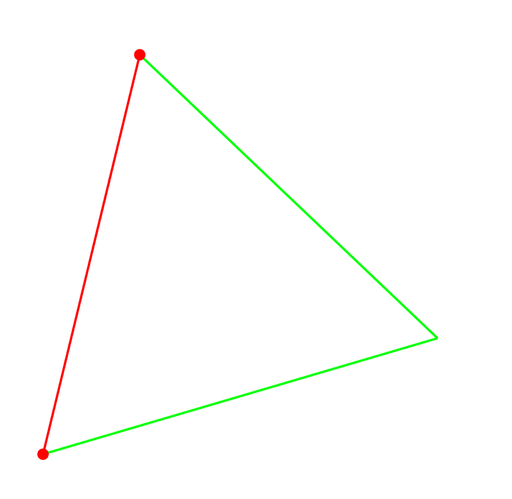
\includegraphics[width = 2.5 in]{img/Equilateral_example/input_image0.png}} &
\subfloat{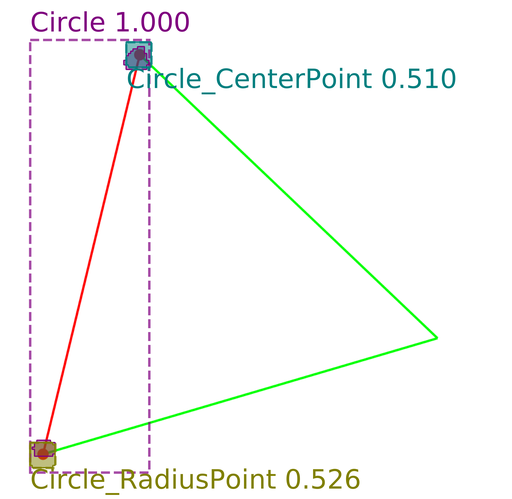
\includegraphics[width = 2.5 in]{img/Equilateral_example/output_image0.png}}\\

 a) Initial configuration & b) Construction step: 1. Based on the prediction a circle will be constructed.\\
 %and first prediction & and second prediction \\

\subfloat{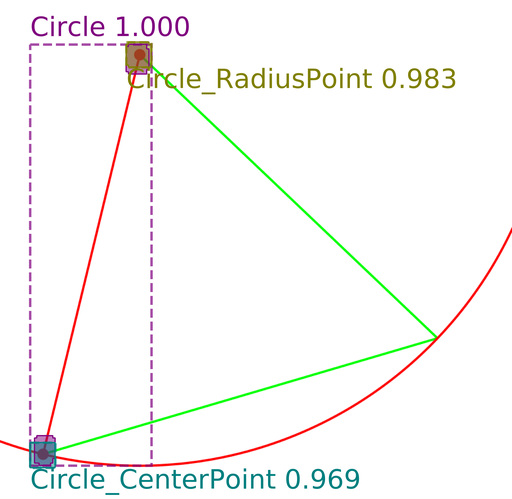
\includegraphics[width = 2.5 in]{img/Equilateral_example/output_image1.png}} &
\subfloat{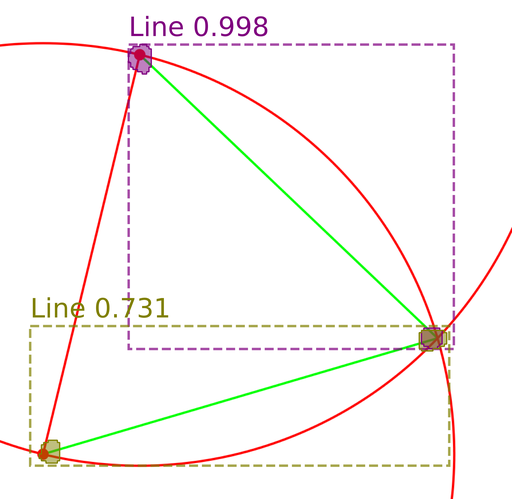
\includegraphics[width = 2.5 in]{img/Equilateral_example/output_image2.png}}\\

c) Construction step: 2. Based on the prediction a circle with a different center then in last step will be constructed.   & d) Construction step: 3. Based on the prediction a line will be constructed. \\[5cm]
%and third prediction & and fourth prediction \\

\subfloat{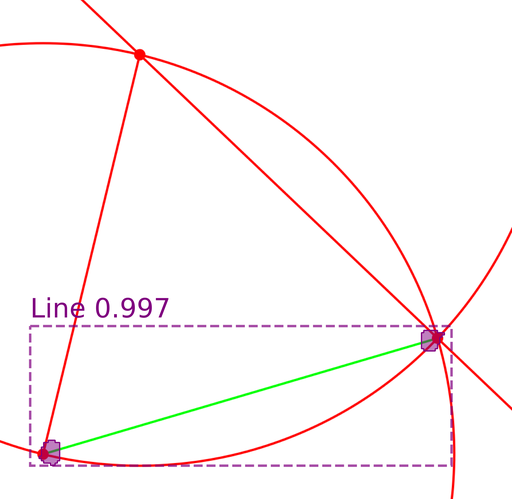
\includegraphics[width = 2.5 in]{img/Equilateral_example/output_image3.png}}&
\subfloat{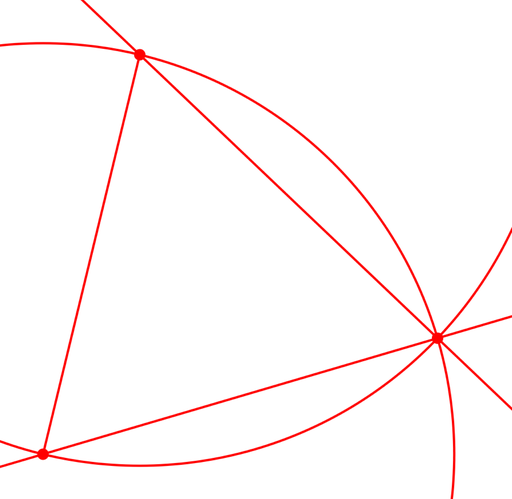
\includegraphics[width = 2.5 in]{img/Equilateral_example/input_image4.png}}\\
e) Construction step: 4. Based on the prediction a line will be constructed. &
f) Construction step: 5 - level finished &\\
%f) construction step: 5 - level finished \\
%and sixth prediction &  \\


\caption{Sequence of construction steps with predictions for the Euclidea level \textbf{Alpha-01} Equilateral Triangle. The first state is the level definition consisting of the initial configuration (red) and the remaining goal (green). In each step, our approach predicts the usage of one tool towards constructing the goal.}
\label{EuclideaExample-Network}
\end{longtable}
